\chapter{Metodología}
\label{ch:methodology}

\section{Flujo general}

El desarrollo siguió un flujo iterativo: definición del contexto y clases,
preparación del dataset, construcción de la aplicación web, integración del proxy
de predicción, entrenamiento del modelo en Custom Vision y validación del producto.
El siguiente diagrama resume el flujo de interacción en la aplicación.

\begin{mermaid}[style=editorial, width=0.95\linewidth, pos=H, caption={Flujo general de predicción en Litoteca}]
  sequenceDiagram
    autonumber
    actor U as Usuario
    participant W as Litoteca Web
    participant F as CF Pages Function
    participant CV as Custom Vision
    participant WK as Wiki cache (build)

    U->>W: Captura o carga imagen
    activate W
    W->>W: Preprocesa y valida imagen
    W->>F: POST /api/predict
    activate F
    F->>CV: Solicita clasificación
    activate CV
    CV-->>F: Predicciones por clase
    deactivate CV
    F-->>W: JSON normalizado (top, confianza, margen)
    deactivate F
    W->>WK: Consulta extracto cacheado
    activate WK
    WK-->>W: Extracto y fuente CC BY-SA
    deactivate WK
    W-->>U: Muestra ficha, confianza, gemelas y contexto
    deactivate W
\end{mermaid}

\section{Selección y preparación del dataset}

\subsection{Fuente}

Se utilizó el dataset \emph{Rock Classification} de Kaggle, exportado originalmente
desde Roboflow~\cite{rockdataset}. El export contenía 4.212 imágenes en 9 clases,
con aumentos sintéticos generados por Roboflow (3 versiones por imagen original:
espejo, recorte, brillo/exposición, entre otros).

La copia local del dataset se mantuvo en \texttt{data/raw/rock-data} y el resultado
preparado en \texttt{data/prepared}. Por tamaño, \texttt{data/} no se versiona en
Git; se documenta su reconstrucción con \texttt{tools/prepare\_dataset.py}.

\subsection{Problemas encontrados}

El análisis inicial detectó dos problemas importantes:

\begin{itemize}
  \item \textbf{Fuga entre splits}: el mismo original aparecía en train y valid/test
        con distintos aumentos. Se encontraron 89 originales compartidos entre train
        y valid, 43 entre train y test, y 15 entre valid y test.
  \item \textbf{Conflictos de etiqueta}: 22 pares de imágenes casi idénticas tenían
        etiquetas distintas, especialmente entre clases síliceas como chert,
        diatomite y siliceous-sinter.
\end{itemize}

\subsection{Limpieza y reconstrucción}

El script \texttt{tools/prepare\_dataset.py} realizó:

\begin{enumerate}
  \item Agrupación por imagen original (cluster), no por archivo aumentado.
  \item Cálculo de hash perceptual \texttt{dHash} para detectar duplicados y
        casi-duplicados.
  \item Reconstrucción de splits sin intersección de clusters: 85/15 estratificado
        para train/valid sobre originales no reservados a test.
  \item En valid/test se conservó un representante por cluster (medoid).
  \item En train se conservaron aumentos del export original.
  \item Generación de manifiestos: \texttt{manifest.csv}, \texttt{stats.json},
        \texttt{conflicts.csv}, \texttt{near\_duplicates.csv}, \texttt{descartadas.csv}.
\end{enumerate}

\begin{table}[H]
  \centering
  \caption{Dataset preparado inicial (con aumentos en train)}
  \label{tab:dataset-prepared}
  \begin{tabular}{@{}lrrrr@{}}
    \toprule
    Clase & Originales & Train & Valid & Test \\
    \midrule
    Basalto & 198 & 398 & 27 & 15 \\
    Basalto olivínico & 192 & 359 & 18 & 19 \\
    Arcilla & 198 & 410 & 26 & 12 \\
    Conglomerado & 200 & 414 & 23 & 13 \\
    Lutita & 195 & 367 & 26 & 20 \\
    Diatomita & 198 & 383 & 22 & 19 \\
    Sílex & 195 & 379 & 21 & 14 \\
    Sinter silíceo & 181 & 354 & 21 & 11 \\
    Yeso & 197 & 364 & 25 & 23 \\
    \midrule
    \textbf{Total} & \textbf{1754} & \textbf{3428} & \textbf{209} & \textbf{146} \\
    \bottomrule
  \end{tabular}
\end{table}

\subsection{Versión limpia para Custom Vision}

Para un nuevo entrenamiento se generó \texttt{data/prepared-clean-train} con la
política: \textbf{una imagen por cluster} en todos los splits, excluyendo clusters
involucrados en conflictos de etiqueta. Los casi-duplicados entre clusters se
marcaron en reporte, pero no se eliminaron automáticamente para evitar una limpieza
demasiado agresiva sin revisión visual.

\begin{table}[H]
  \centering
  \caption{Dataset limpio usado para el nuevo entrenamiento}
  \label{tab:dataset-clean}
  \begin{tabular}{@{}lrrr@{}}
    \toprule
    Clase & Train & Valid & Test \\
    \midrule
    Basalto & 156 & 27 & 15 \\
    Sílex & 148 & 21 & 14 \\
    Arcilla & 152 & 26 & 12 \\
    Conglomerado & 155 & 23 & 13 \\
    Diatomita & 145 & 22 & 19 \\
    Yeso & 144 & 25 & 23 \\
    Basalto olivínico & 143 & 18 & 19 \\
    Lutita & 145 & 26 & 20 \\
    Sinter silíceo & 137 & 21 & 11 \\
    \midrule
    \textbf{Total} & \textbf{1325} & \textbf{209} & \textbf{146} \\
    \bottomrule
  \end{tabular}
\end{table}

Esta versión reduce redundancia sintética y evita que el modelo aprenda artefactos
de aumentos del export. Custom Vision puede aplicar sus propias transformaciones de
entrenamiento; por eso se prefirió subir imágenes limpias.

\section{Entrenamiento del modelo}

El entrenamiento se realiza en Azure Custom Vision. Se creó un proyecto multiclase
de Litoteca y se cargaron las imágenes por etiqueta. Se probaron dos enfoques:

\begin{itemize}
  \item \textbf{Iteración avanzada inicial}: entrenamiento largo en el proyecto
        original; la ejecución permaneció en estado de entrenamiento por más de 13
        horas, por lo que se decidió validar con un proyecto limpio.
  \item \textbf{Proyecto limpio, entrenamiento Quick}: se creó el proyecto
        \texttt{litoteca-clean-quick}, se cargaron 1534 imágenes (train+valid
        limpios, 1 por cluster, conflictos excluidos) y se completó un entrenamiento
        Quick. La iteración obtuvo precisión 83.08\%, recall 52.43\% y AP 72.74\%;
        se puede usar como base para la demo mientras se prueba una iteración mejorada.
\end{itemize}

Las credenciales y endpoints de predicción se manejan como variables de entorno en
Cloudflare Pages, no en el frontend.

\section{Desarrollo de la aplicación}

\subsection{Arquitectura}

La aplicación es un sitio estático sin build: HTML, CSS y JavaScript vanilla. La
predicción se consume mediante una Cloudflare Pages Function en
\texttt{functions/api/predict.js}, que recibe la imagen, la envía a Custom Vision y
normaliza la respuesta al contrato de Litoteca.

\begin{table}[H]
  \centering
  \caption{Componentes principales de la aplicación}
  \label{tab:componentes}
  \begin{tabular}{@{}p{3.6cm}p{8.8cm}@{}}
    \toprule
    Componente & Responsabilidad \\
    \midrule
    \texttt{index.html} & Estructura de vistas: inicio, cámara, resultado, historial. \\
    \texttt{assets/app.js} & Lógica de UI, cámara, subida, mock, historial local. \\
    \texttt{assets/app.css} & Sistema visual editorial/papel. \\
    \texttt{assets/fichas.js} & Fichas curadas de las 9 clases. \\
    \texttt{functions/api/predict.js} & Proxy a Custom Vision, validación y contrato. \\
    \texttt{sw.js} & Service worker para modo sin conexión honesto. \\
    \texttt{scripts/gates.sh} & Gates deterministas y pruebas de navegador. \\
    \bottomrule
  \end{tabular}
\end{table}

\subsection{Interfaz de usuario}

La interfaz se diseñó con enfoque móvil, accesible y educativo. Incluye:

\begin{itemize}
  \item Captura con cámara o carga de imagen.
  \item Vista de resultado con clase, confianza, margen y alternativas.
  \item Fichas con explicación: qué es, cómo se formó, gemelas y señales.
  \item Historial local en el navegador.
  \item Modo demostración con \texttt{?mock=1} y \texttt{?galeria=1}.
  \item Modo sin conexión para recursos ya cacheados; la predicción en línea se
        desactiva cuando no hay red.
\end{itemize}

\subsection{Generación de ilustraciones}

Para reforzar el valor pedagógico, se generaron ilustraciones del proceso geológico
de cada roca. Las ilustraciones se produjeron con \texttt{facet + ComfyUI}
(workflow \texttt{flux2-klein-4b}) a partir de una pieza reproducible
(\texttt{tools/procesos-geologicos.toml}). Luego se optimizaron a WebP/PNG y se les
agregaron etiquetas de texto reales manualmente, evitando texto sintético generado
por el modelo de imagen.

\begin{figure}[H]
  \centering
  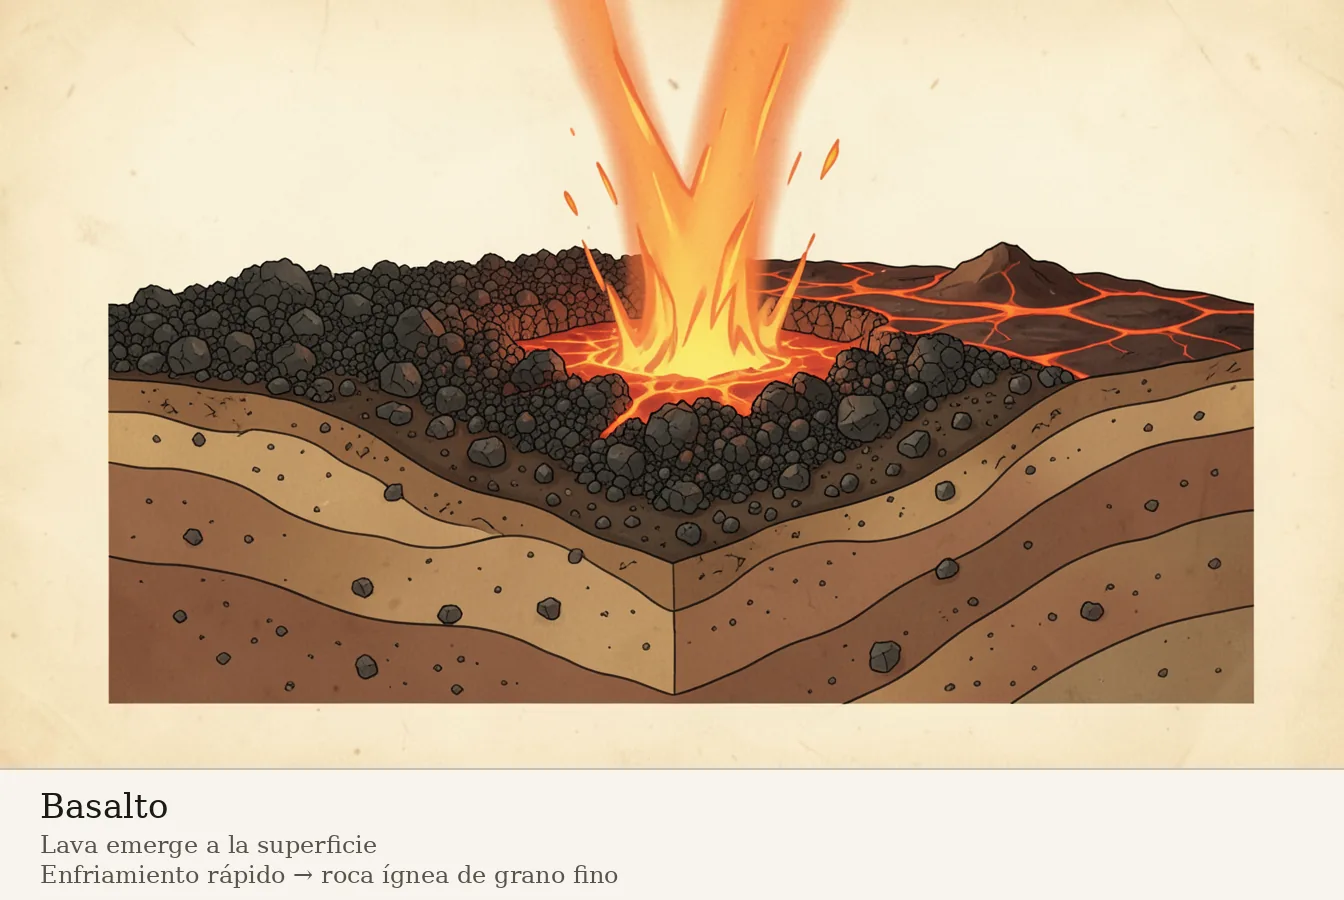
\includegraphics[width=0.82\linewidth]{assets/images/basalt.png}
  \caption{Ejemplo de ilustración generada para el proceso de formación del basalto}
  \label{fig:basalt}
\end{figure}

\section{Despliegue}

La aplicación se despliega en Cloudflare Pages. El flujo de despliegue usa GitHub
Actions con \texttt{workflow\_dispatch} desde la rama \texttt{develop}, entorno
\texttt{production}, y \texttt{wrangler pages deploy}. Los secretos de Cloudflare se
configuran en GitHub Environment secrets; los secretos de Custom Vision se
configuran en Cloudflare Pages como variables de runtime de la Function.

La versión actual está disponible en \url{https://litoteca.pages.dev/}.
